\documentclass[letter,10pt]{article}
\usepackage[letterpaper, lmargin=.5in, rmargin=.5in, tmargin=.5in]{geometry}
\usepackage[utf8]{inputenc}
\usepackage{verbatim}
\usepackage{color}
\usepackage[]{amsmath}
\usepackage{mathtools}
\usepackage{pdfpages}
\usepackage{enumitem}
\usepackage{listings}
\usepackage{amssymb}
\usepackage{amsfonts}
\usepackage{graphicx}
\usepackage{subfig}
% \usepackage{pstool}
\usepackage{algorithm}
\usepackage{array}
\usepackage{tikz}
\usetikzlibrary{matrix}
\usepackage[binary-units]{siunitx}
\usepackage[backref=page,
            pageanchor=true,
            plainpages=false,
            pdfpagelabels,
            bookmarks,
            bookmarksnumbered,
            linkbordercolor={1 0.5 0.5},
            citebordercolor={0 0.5 0},
]{hyperref}

\usepackage{array,mathtools}
\newcommand*{\carry}[1][1]{\overset{#1}}
\newcolumntype{B}[1]{r*{#1}{@{\,}r}}

\newcommand{\eg}{\textit{e.g.},~}
\newcommand{\etc}{\textit{etc.}}
\let\eqref\undefined

\newcommand{\figref}[1]{Figure~\ref{fig:#1}}
\newcommand{\algoref}[1]{Algorithm~\ref{algo:#1}}
\newcommand{\secref}[1]{Section~\ref{sec:#1}}
\newcommand{\tabref}[1]{Table~\ref{tab:#1}}
\newcommand{\eqref}[1]{Equation~\ref{eq:#1}}
\newcommand{\figlabel}[1]{\label{fig:#1}}
\newcommand{\algolabel}[1]{\label{algo:#1}}
\newcommand{\seclabel}[1]{\label{sec:#1}}
\newcommand{\tablabel}[1]{\label{tab:#1}}
\newcommand{\eqlabel}[1]{\label{eq:#1}}

\DeclarePairedDelimiter\abs{\lvert}{\rvert}%
\DeclarePairedDelimiter\norm{\lVert}{\rVert}%


% Title Page
\title{CMPSCI 453\\HW9, Wireshark Lab 5}
\author{Tony Gao}

\begin{document}
\maketitle

%\begin{abstract}
%\end{abstract}

\section{Lab}

\begin{enumerate}	
	\item The source IP is 192.168.1.102. The source port is 1161.
	
	\begin{verbatim}
	1 0.000000       192.168.1.102         128.119.245.12        TCP      62     1161 -> 80
	[SYN] Seq=0 Win=16384 Len=0 MSS=1460 SACK_PERM=1
	Frame 1: 62 bytes on wire (496 bits), 62 bytes captured (496 bits)
	Ethernet II, Src: PremaxPe_8a:70:1a (00:20:e0:8a:70:1a), Dst: LinksysG_da:af:73 (00:06:25:da:af:
	73)
	Internet Protocol Version 4, Src: 192.168.1.102, Dst: 128.119.245.12
	Transmission Control Protocol, Src Port: 1161, Dst Port: 80, Seq: 0, Len: 0
	\end{verbatim}
	
	\item The IP of gaia.cs.umass.edu is 128.119.245.12. The port is 80.
	
	\item The IP of the client in my user-generated trace is 10.0.0.157, the port is 56564.
	
		\begin{verbatim}
	314 14.494856      10.0.0.157            128.119.245.12        TCP      66     56564 -> 80
	[ACK] Seq=1 Ack=1 Win=131744 Len=0 TSval=287860679 TSecr=1425403752
	Frame 314: 66 bytes on wire (528 bits), 66 bytes captured (528 bits) on interface 0
	Ethernet II, Src: Apple_10:41:06 (80:e6:50:10:41:06), Dst: ArrisGro_0f:07:81 (10:56:11:0f:07:81)
	Internet Protocol Version 4, Src: 10.0.0.157, Dst: 128.119.245.12
	Transmission Control Protocol, Src Port: 56564, Dst Port: 80, Seq: 1, Ack: 1, Len: 0
	\end{verbatim}
	
	\item The sequence number of the SYN segment is 0. The TCP header flag field bitmask 0x002 denotes a SYN segment.
	
	\begin{verbatim}
	Flags: 0x002 (SYN)
	000. .... .... = Reserved: Not set
	...0 .... .... = Nonce: Not set
	.... 0... .... = Congestion Window Reduced (CWR): Not set
	.... .0.. .... = ECN-Echo: Not set
	.... ..0. .... = Urgent: Not set
	.... ...0 .... = Acknowledgment: Not set
	.... .... 0... = Push: Not set
	.... .... .0.. = Reset: Not set
	.... .... ..1. = Syn: Set
	.... .... ...0 = Fin: Not set
	[TCP Flags: ··········S·]
	\end{verbatim}
	
	\item The sequence number of the SYNACK is 0. The ACK number is 1. The server determines this by taking the sequence number of the syn segment plus 1. The bitmask 0x010 $|$ 0x002 = 0x012 denotes syn + ack in the TCP header flags. 
	
	\begin{verbatim}
	Flags: 0x012 (SYN, ACK)
	000. .... .... = Reserved: Not set
	...0 .... .... = Nonce: Not set
	.... 0... .... = Congestion Window Reduced (CWR): Not set
	.... .0.. .... = ECN-Echo: Not set
	.... ..0. .... = Urgent: Not set
	.... ...1 .... = Acknowledgment: Set
	.... .... 0... = Push: Not set
	.... .... .0.. = Reset: Not set
	.... .... ..1. = Syn: Set
	.... .... ...0 = Fin: Not set
	[TCP Flags: ·······A··S·]
	
	\end{verbatim}
	
	\item The sequence number of the segment containing the POST is 1
	
	\begin{verbatim}
	4	0.026477	192.168.1.102	128.119.245.12	TCP	619	1161 -> 80 [PSH, ACK] Seq=1 Ack=1 Win=17520 Len=565 [TCP segment of a reassembled PDU]
	%s pE]!@fwP
4tPDpPOST /ethereal-labs/lab3-1-reply.htm HTTP/1.1
	Host: gaia.cs.umass.edu
	User-Agent: Mozilla/5.0 (Windows; U; Windows NT 5.1; en-US; rv:1.0.2) Gecko/20030208 Netscape/7.02
	Accept: text/xml,application/xml,application/xhtml+xml,text/html;q=0.9,text/plain;q=0.8,video/x-mng,image/png,image/jpeg,image/gif;q=0.2,text/css,*/*;q=0.1
	Accept-Language: en-us, en;q=0.50
	Accept-Encoding: gzip, deflate, compress;q=0.9
	Accept-Charset: ISO-8859-1, utf-8;q=0.66, *;q=0.66
	Keep-Alive: 300
	Connection: keep-alive
	Referer: http://gaia.cs.umass.edu/ethereal-labs/lab3-1.htm
	\end{verbatim}
	
	\item First six segments starting from HTTP Post as first segment: 
		\begin{itemize}
			\item Sequence 1, time sent: 0.026477000s, ack 566 received 0.053937000s. RTT=27.46ms, len 565
			\item Sequence 566 sent:  0.041737000s, ack 2026 received: 0.077294000s. RTT=35.557ms, len 1460
			\item Sequence 2026 sent:  0.054026000s, ack 3486 received: 0.124085000s RTT=70.059ms, len 1460
			\item Sequence 3486 sent:  0.054690000s, ack 4946 received: 0.169118000s RTT=114.428ms, len 1460
			\item Sequence 4946 sent:  0.077405000s, ack 6406 received: 0.217299000s RTT=139.894ms, len 1460
			\item Sequence 6406 sent: 0.078157000s, ack 7866 received: 0.267802000s RTT=189.645ms, len 1460
		\end{itemize}
		\begin{itemize}
			\item $EstimatedRTT_0$ = 27.46ms 
			\item $EstimatedRTT_1$ = $.875 \cdot 27.46 + .125 \cdot 35.557$ = 28.472125ms
			\item $EstimatedRTT_2$ = $.875 \cdot 28.472125 + .125 \cdot 70.059$  = 33.670484375ms
			\item $EstimatedRTT_3$ = $.875 \cdot 33.670484375 + .125 \cdot 114.428$ = 43.765173828125ms
			\item $EstimatedRTT_4$ = $.875 \cdot 43.765173828125 + .125 \cdot 139.894$ = 55.781277099609375ms
			\item $EstimatedRTT_5$ = $.875 \cdot 55.781277099609375 + .125 \cdot 189.645$ = 72.514242462158203125ms
		\end{itemize}
	
	\item First six segment lengths:
		\begin{itemize}
			\item Sequence 1 len 565
			\item Sequence 566 len 1460
			\item Sequence 2026 len 1460
			\item Sequence 3486 len 1460
			\item Sequence 4946 len 1460
			\item Sequence 6406 len 1460
		\end{itemize}
	\item The minimum receiver buffer space is advertised in capture packet number 2. It is 5840B. This does not throttle the sender speed because the receiver window size grows faster than the total amount of unacked packets. Total unacked packets reaches a maximum of 6, but receiver window continues to grow far past 6 * 1460B. When the TCP connection is in Slow Start, the receiver window is approximately double the size of the total amount of unacked packets, which means the receiver still has space to buffer more packets, but the sender congestion window size does not allow for any more packets.
	
	\begin{verbatim}
	Transmission Control Protocol, Src Port: 80, Dst Port: 1161, Seq: 0, Ack: 1, Len: 0
	Source Port: 80
	Destination Port: 1161
	[Stream index: 0]
	[TCP Segment Len: 0]
	Sequence number: 0    (relative sequence number)
	Acknowledgment number: 1    (relative ack number)
	0111 .... = Header Length: 28 bytes (7)
	Flags: 0x012 (SYN, ACK)
	Window size value: 5840
	[Calculated window size: 5840]
	Checksum: 0x774d [unverified]
	[Checksum Status: Unverified]
	Urgent pointer: 0
	Options: (8 bytes), Maximum segment size, No-Operation (NOP), No-Operation (NOP), SACK permitted
	[SEQ/ACK analysis]
	\end{verbatim}
	
	\item There are no retransmissions. This is observed by setting the display filter to "tcp and (tcp.analysis.retransmission or tcp.analysis.fast\_retransmission)" and seeing an empty packet display window.
	
	\item Sequence 41781 (len 1460, ack num 43241) and 43241(len 1460, ack num 44701) were sent back to back, and the receiver only acks 44701, which is the ack number for sequence 43241. The receiver typically acknowledges 1460B in an ack.
	\pagebreak
	
	\item The average throughput seems to be approximately 225000 b/s = 28125 B/s = 28.125 KB/s over a  ~5 second time interval.
		\begin{center}
			\noindent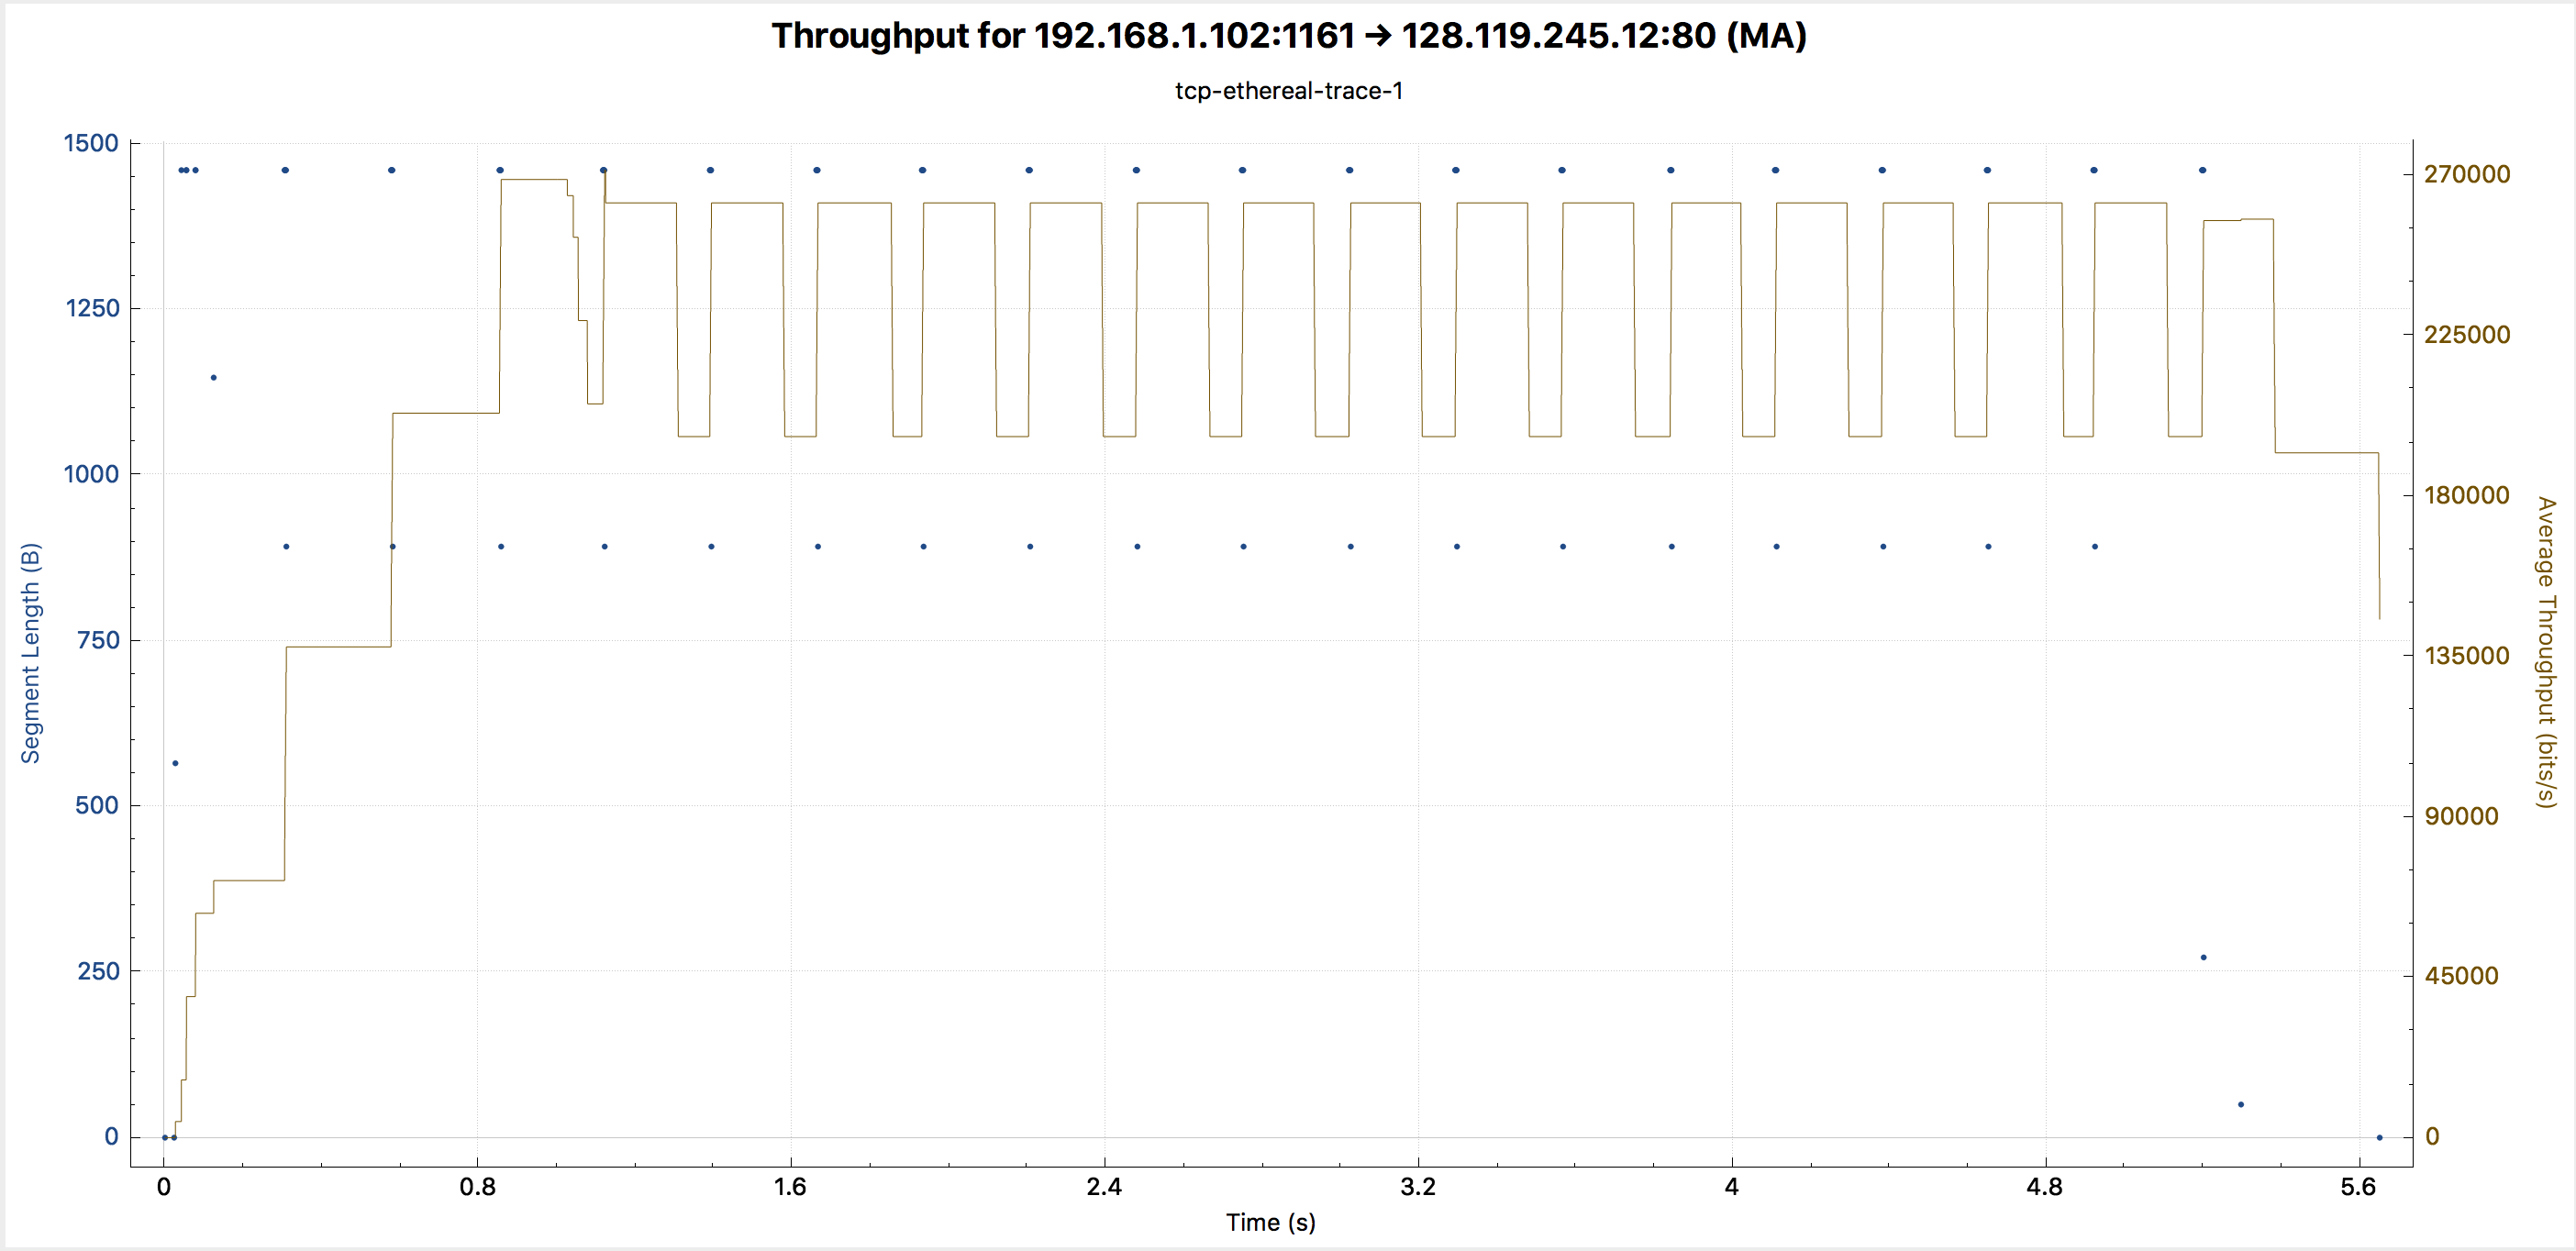
\includegraphics[height=.5\textheight,width=.9\textwidth]{./figures/hw9p12}
		\end{center}
	\pagebreak
	
	\item Slow start begins with the syn segment, the first segment sent. Slow start ends after sequence number 7866 is received (ack 9013). Congestion avoidance takes over starting from sequence 9013. Congestion avoidance ends after sequence 163769 is sent, which is the end of alice.txt. The TCP congestion avoidance behavior seen in the graph seems to max out at 6 unacked sequences at a time. In the ideal TCP, the number of unacked segments would grow by 1 MSS per RTT, so a sequence of [5, 6, 7, ...] unacked segments would be seen until either three duplicate acks are received or a timeout event occurs, at which point fast recovery would be entered and the congestion window would be decreased depending on which recovery algorithm is used. Instead, the congestion window seems to be a constant size. The maximum unacked segment size does not seem to be influenced by flow control, because the receiver window is much larger than $5 \cdot 1460$.
		\begin{center}
		\noindent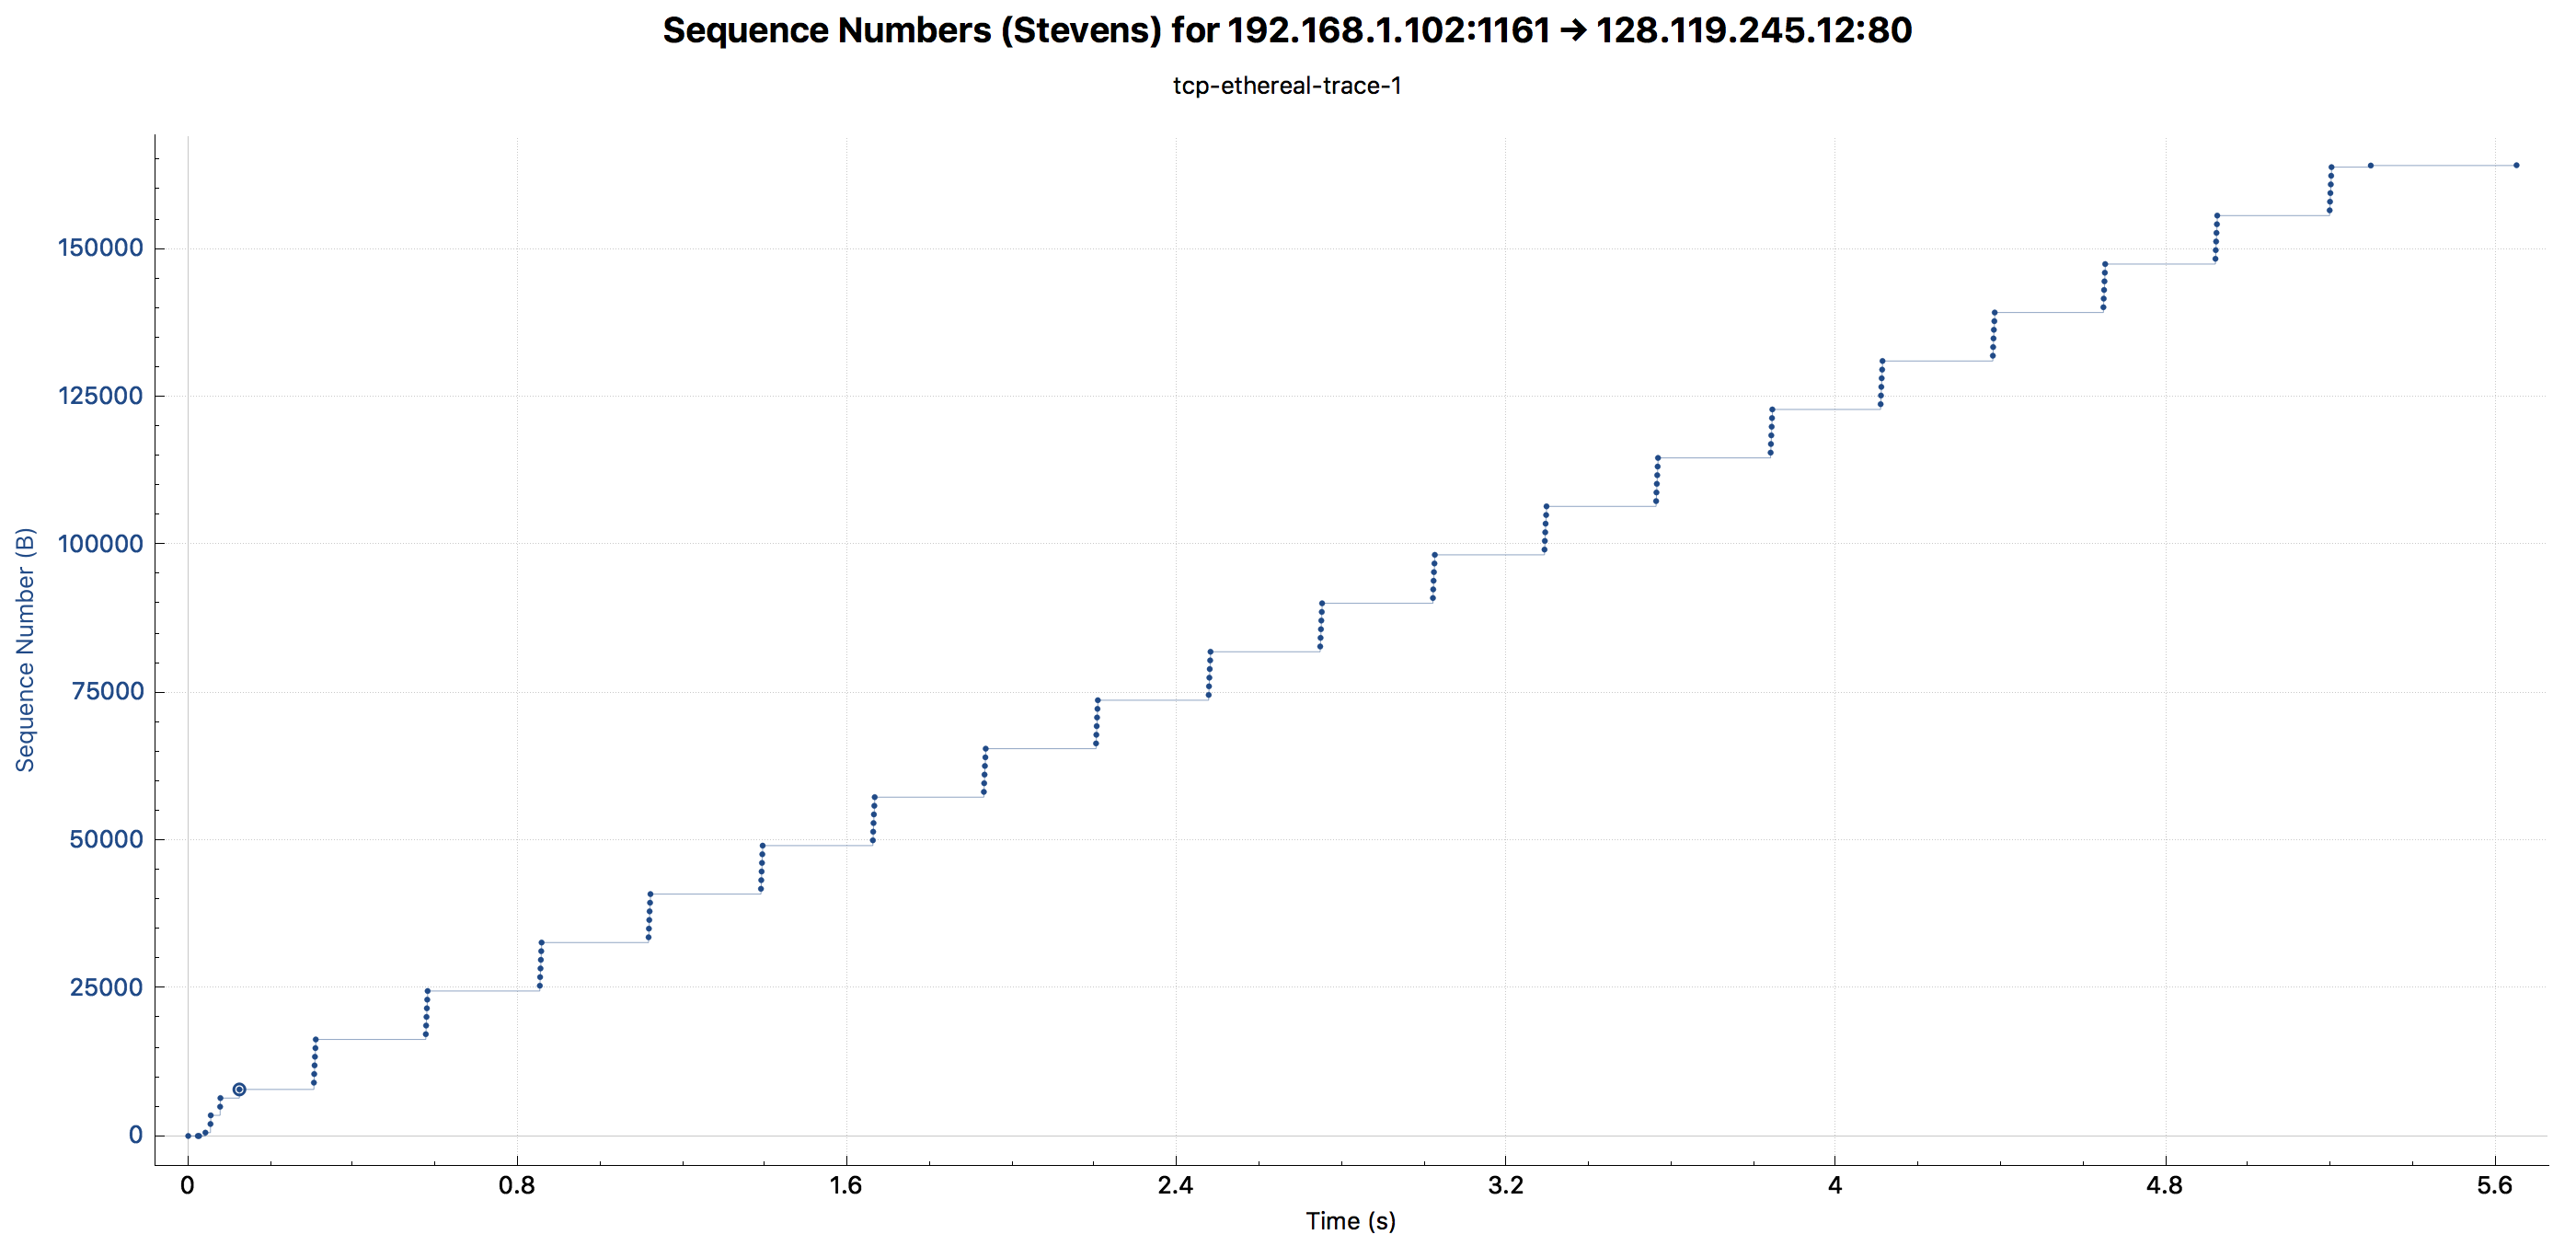
\includegraphics[height=.5\textheight,width=.9\textwidth]{./figures/hw9p13}
		\end{center}
	\pagebreak
	
	\item Slow start begins with the first segment sent. Slow start ends after segment 152716 is sent. The average throughput is approximately 700000 b/s = 87500 B/s = 87.5 KB/s over a 1.5s interval. The congestion window seems to grow exponentially until all the alice.txt file bytes are done transferring. There are no error events. Congestion avoidance and Fast recovery are never entered. This seems to closely mirror ideal TCP slow start behavior. My computer appears to have a slow start implementation similar to the reference algorithm suggested in RFC2001, as the slow start threshold appears to be large, at least 65535B. RFC5681 suggests a ssthresh as big as the largest possible rwnd.  In the graph, it is clear that on the the command window size continued to double past the reference threshold suggested by RFC2001. ~66 sequences are sent from T=.5s to T=.65s back to back. By looking at the wireshark packet capture listing, I see that the acks for those sequences do not begin to arrive until nearly all the sequences are sent, meaning the congestion window is on the order of $2^{log_2(66 \cdot 1460)} \approx 2^{17}$ bytes large at this point. If the file was larger, maybe my computer would have entered congestion avoidance sometime past this point. It is impossible to tell if there are any differences in congestion avoidance between my computer's TCP implementation and the ideal because congestion avoidance is never entered.
	\begin{center}
		\noindent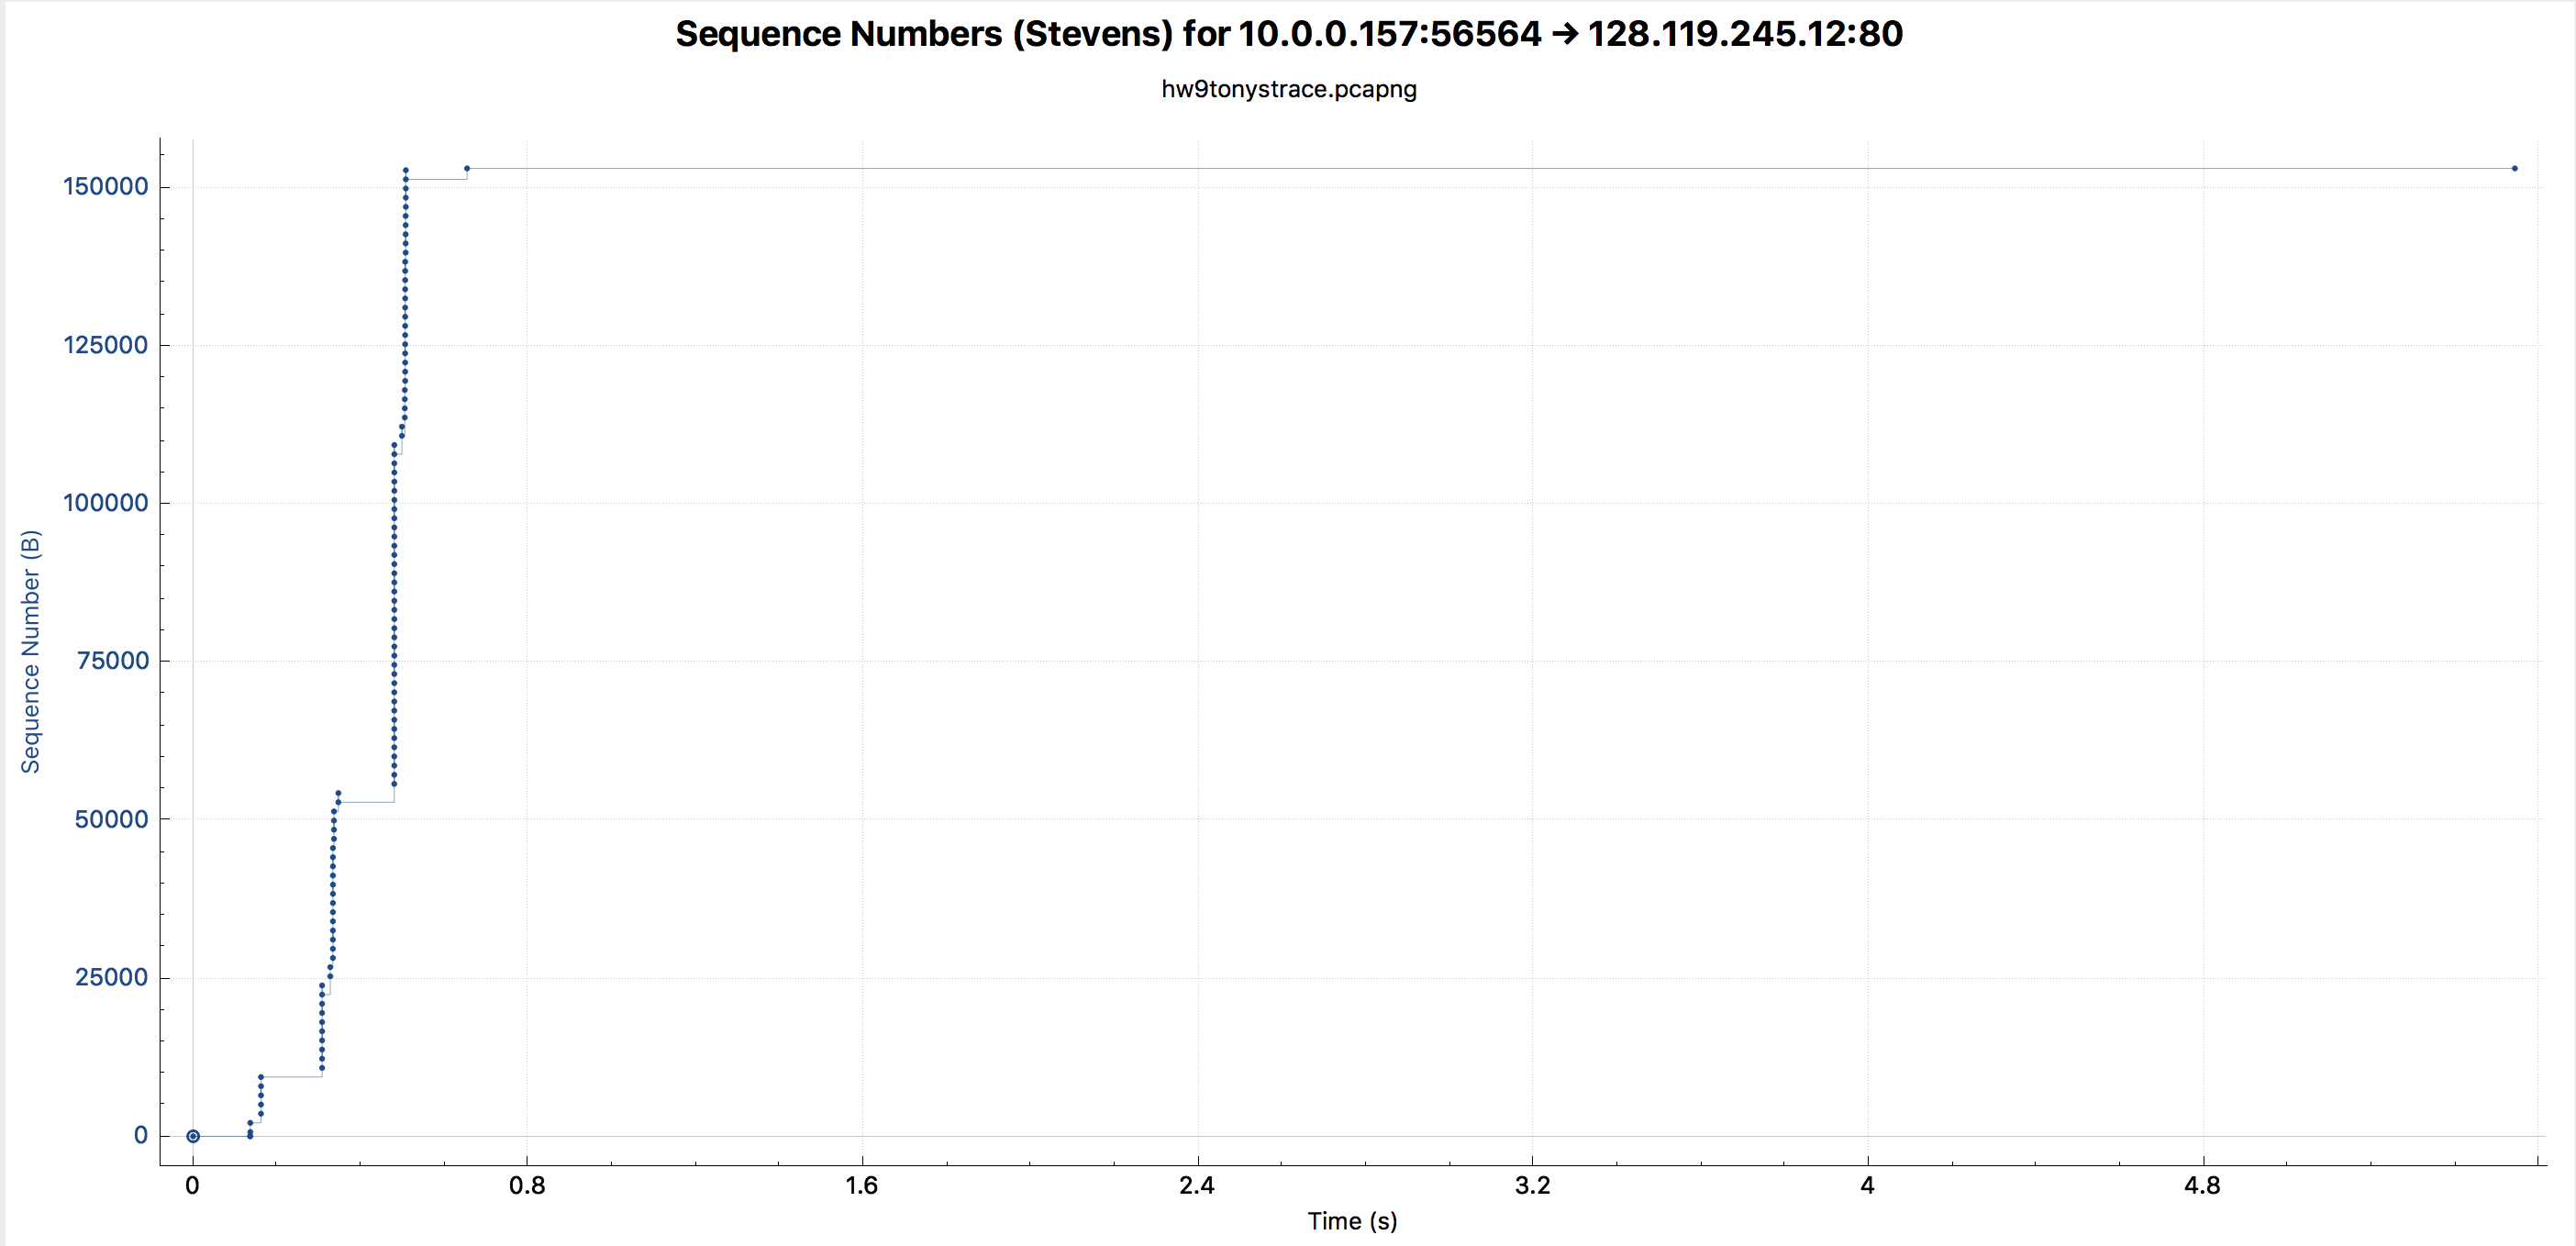
\includegraphics[height=.5\textheight,width=.9\textwidth]{./figures/hw9p14segments}
	\end{center}
	\begin{center}
		\noindent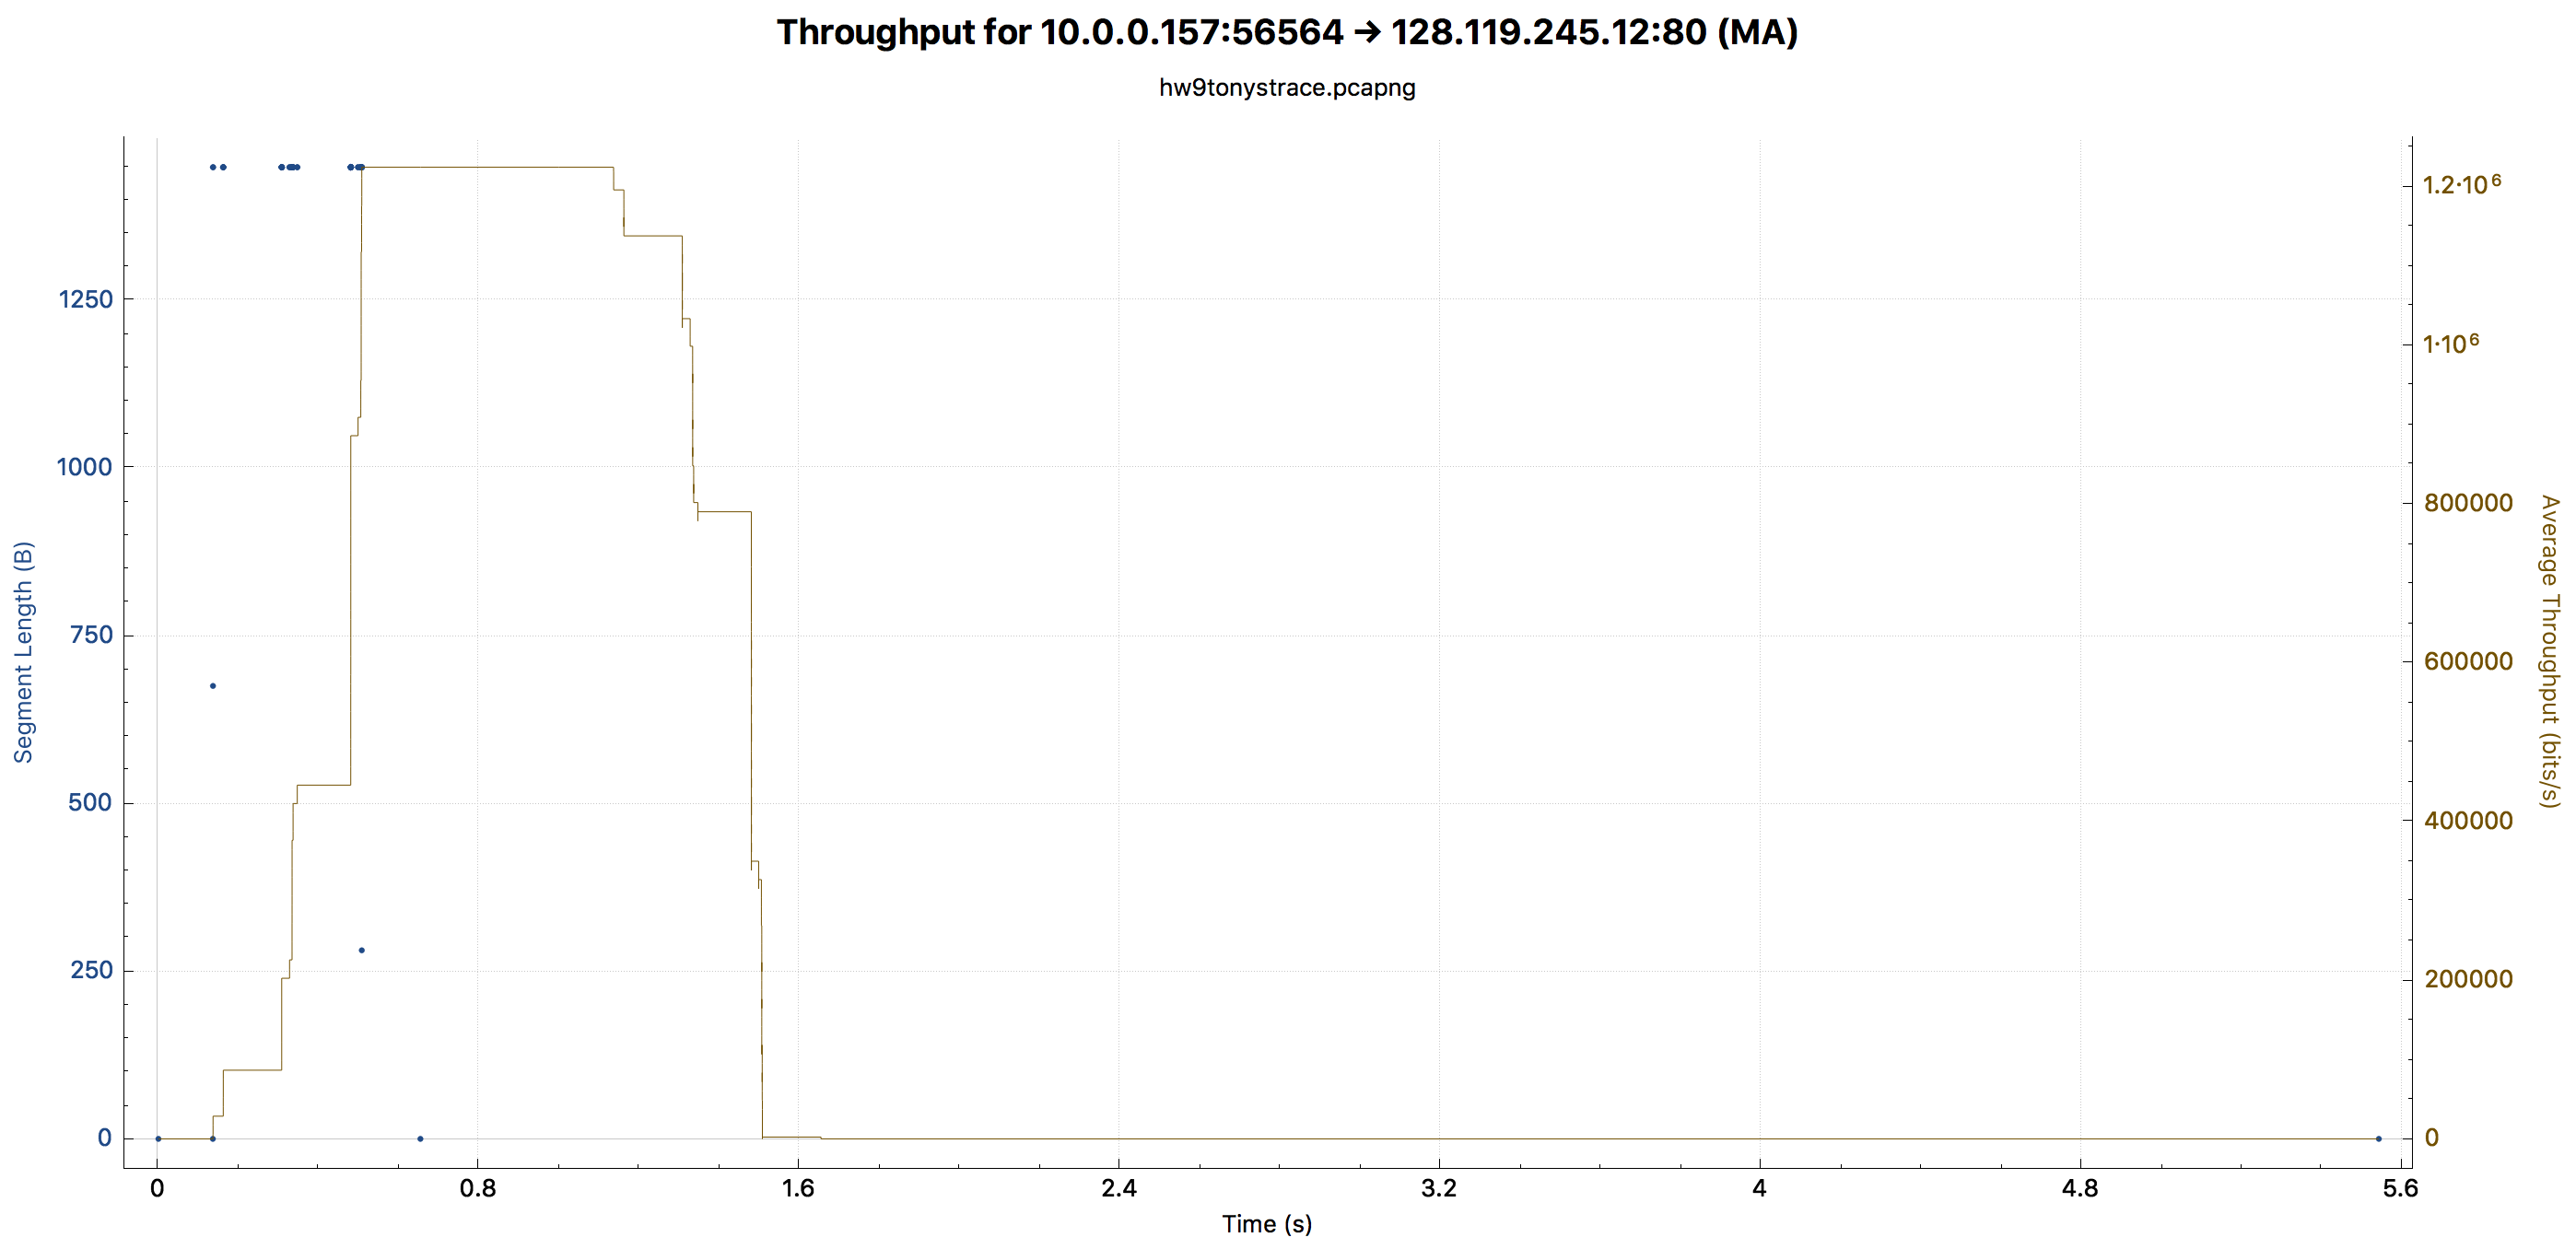
\includegraphics[height=.5\textheight,width=.9\textwidth]{./figures/hw9p14throughput}
	\end{center}
\end{enumerate}



\end{document}
